\documentclass[11pt,twocolumn,twoside]{opticajnl}
%% Please use 11pt if submitting to AOP
% \documentclass[11pt,twocolumn,twoside]{opticajnl}

\journal{pr} % Choose journal (ao,jocn,josaa,josab,ol,optica,pr)

%See template introduciton for guidance on setting shortarticle option
\setboolean{shortarticle}{True}
% true = letter/tutorial
% false = research/review article
% (depending on journal)
\usepackage{lineno}
\usepackage[utf8]{inputenc}
\spanishdecimal{.}
\usepackage{amsmath}
\usepackage{caption}
\usepackage{subcaption}
\usepackage[spanish]{babel}
\usepackage{hyperref}
\usepackage{listings}
\usepackage{multicol}
%\linenumbers

% Configura el formato del título del listado
\renewcommand\lstlistingname{Código}
\renewcommand\lstlistlistingname{Códigos}
\title{

\vspace{0.5cm} 

Trabajo práctico 1: Dinámica de sistemas acoplados}

\author[1]{\huge{Ignacio Lembo Ferrari}}
\affil[1]{\large{ignaciolembo@ib.edu.ar} 

\vspace{0.3cm}

\large{13 de septiembre de 2023.}

\vspace{0.5cm}
}

%\begin{abstract}
%\textbf{hola}
%\end{abstract}

\begin{document}

\maketitle

\section{Dinámica de sistemas acoplados \label{sec:p1}}

\vspace{0.3cm}

\subsection{Modelo de Hodgkin y Huxley \label{sec:modelo}}

\vspace{0.3cm}

El modelo de Hodgkin y Huxley consiste en un conjunto de cuatro ecuaciones diferenciales ordinarias no lineales que describen el comportamiento del potencial de una neurona
\begin{align}
    \begin{split}
        C \frac{d V}{d t} &= I_{ext} - g_{K}n^4(V-V_{K}) - \\
                          &~~~~g_{Na}m^3h(V-V_{Na})  - g_{Cl}(V-V_{Cl}), 
        \label{ec:corriente}
    \end{split} \\
    \frac{dn}{dt} &= \frac{n_{\infty}(V) - n}{\tau_n(V)}, \\
    \frac{dm}{dt} &=\frac{m_{\infty}(V) - m}{\tau_m(V)}, \\
    \frac{dh}{dt} &= \frac{h_{\infty}(V) - h}{\tau_h(V)}, 
\end{align}
donde $\tau_x$ y $x_{\infty}$ para $x=n,m,h$ están dados por 
\begin{equation}
    x_{\infty}(V) = \frac{a_x}{a_x+b_x}, \hspace{1cm} \tau_x = \frac{1}{a_x + b_x},
\end{equation}
con $\tau_x$ en milisegundos. Los valores de $a_x$ y $b_x$ están dados por
\begin{align}
    &a_n = \frac{0.01 (V+55)}{1 - \exp[ (-V-55) / 10 ]}, \\
    &b_n = 0.125\exp[ (-V-65)/80], \\
    &a_m = \frac{0.1 (V+40)}{1 - \exp[ (-V-40) / 10 ]}, \\
    &b_m = 4 \exp[ (-V - 65)/18 ], \\
    &a_h = 0.07 \exp[ (-V - 65)/20 ], \\
    &b_h = \frac{1}{1 + \exp[ (-V-35)/10 ]},
\end{align} 
con el potencial $V$ expresado en milivolts. Además los potenciales de inversión y las conductancias máximas están dados por: $V_{Na} = 50$ mV,  $V_{K} = -77$ mV,  $V_{Cl} = -54.4$ mV, $g_{Na} = 120$ mS$/$cm$^2$, $g_{K} = 36$ mS$/$cm$^2$, $g_{Cl} = 0.3$ mS$/$cm$^2$. Además, la capacitancia de la membrana es $C = 1~\mu\text{F}/\text{cm}^2$.

\subsection{Dinámica de dos neuronas}

\vspace{0.3cm}

Se simuló la dinámica de dos neuronas de Hodgkin y Huxley (neurona 1 y neurona 2) conectadas simétricamente con interacciones sinápticas exitatorias ó inhibitorias. Para cada neurona se utilizaron las ecuaciones y los parámetros descriptos en la sección \ref{sec:modelo}. La corriente de interacción sináptica para cada neurona está dada por 
\begin{equation}
    I_{syn} = -g_{syn}~ s(t) (V-V_{syn}),
    \label{ec:Isyn}
\end{equation}
donde
\begin{equation}
    \frac{ds}{dt} = \frac{s_{\infty}(V_{pre}) - s}{\tau},
\end{equation}
con $s_{\infty} = 0.5 ~(1 + \tanh(V/5))$, $\tau = 3$ ms y donde $V_{pre}$ refiere al potencial de la neurona presináptica, es decir, para la neurona 1 es el potencial de la neurona 2 y viceversa. Para la interacción exitatoria se utilizó $V_{syn}= 0$ y para la inhibitoria $V_{syn} = -80$ mV. Se fijó la corriente externa en $I_{ext} = 10 ~\mu\text{A}/\text{cm}^2$ de manera que las neuronas oscilen periódicamente. 

Matemáticamente, la interacción sináptica consiste en sumar la corriente $I_{syn}$ dada por la Ec. (\ref{ec:Isyn}) en el miembro derecho de la Ec. (\ref{ec:corriente}) para cada neurona. De esta manera se tiene, para cada neurona, un sistema de 5 ecuaciones diferenciales acopladas con variables $n$, $m$, $h$, $s$, $V$ y variable independiente el tiempo $t$. Esto resulta en un sistema de 10 ecuaciones diferenciales que se resuelven todas al mismo tiempo con el metodo RK4 implementado en Python. 

Se tomó como condición inicial para la neurona 1: $V(0) = V_K$, $n(0) = n(V_K)$, $m(0) = m(V_K)$, $h(0) = h(V_K)$ y $s(0) = s(V_K)$. Para la neurona 2: $V=0$ mV y $n=m=h=s=0$.

\newpage

En la Fig. \ref{fig:V_vs_t_sinacople} se muestra el caso en que las dos neuronas no es están acopladas ($g_{syn} = 0 ~\text{mS}/\text{cm}^2$). En este caso cada neurona se comporta de manera independiente y el desfasaje entre ambas señales es debido a las diferentes condiciones iniciales de cada neurona.

\begin{figure}[ht]
    \centering
         \begin{subfigure}[b]{\linewidth}
            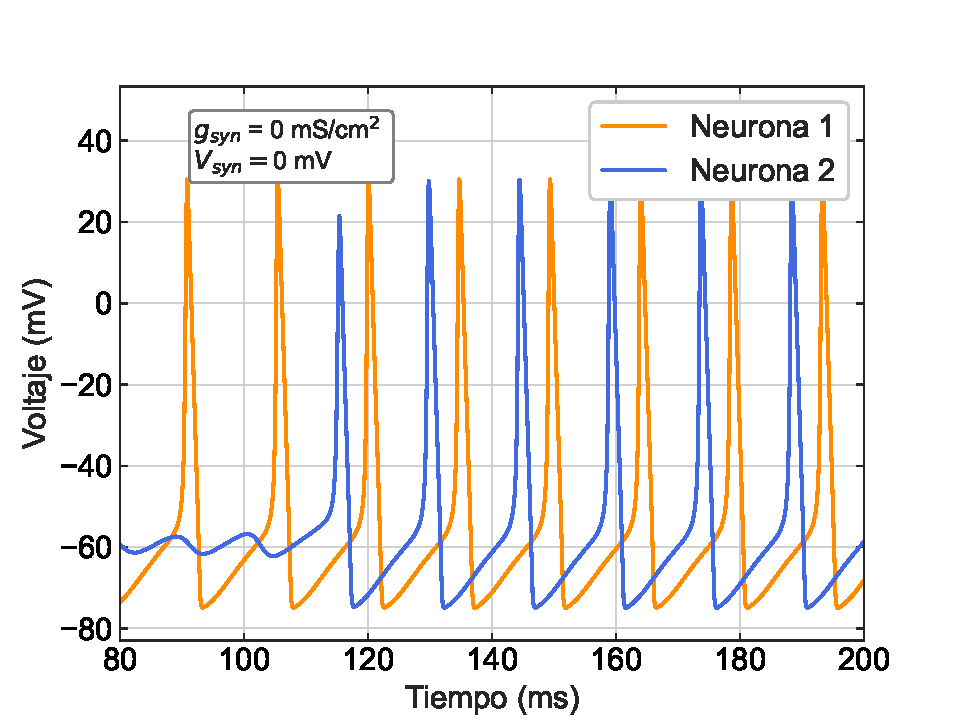
\includegraphics[width=\textwidth]{Figuras/V_vs_t_0_0.pdf}
         \end{subfigure}
    \caption{Potencial de las neuronas 1 y 2 en función del tiempo sin acople sináptico $g_{syn} = 0 \text{mS}/\text{cm}^2$.} 
    \label{fig:V_vs_t_sinacople}
\end{figure}

Se graficó el potencial de las neuronas 1 y 2 en función del tiempo para un acople sinóptico $g_{syn} = 1~\text{mS}/\text{cm}^2$ en el caso de interacción sináptica exitatoria $V_{syn}=0 $ mV (Fig. \ref{fig:V_vs_t_conacople_ext}) e interacción sináptica inhibitoria $V_{syn}= -80$ mV (Fig. \ref{fig:V_vs_t_conacople_inh}). Se observa que luego de un periodo transitorio ambas neuronas se sincronizan. En el caso exitatorio se acoplan en fase y en el inhibitorio en contrafase.

\begin{figure}[H]
\centering
    \begin{subfigure}[b]{\linewidth}
        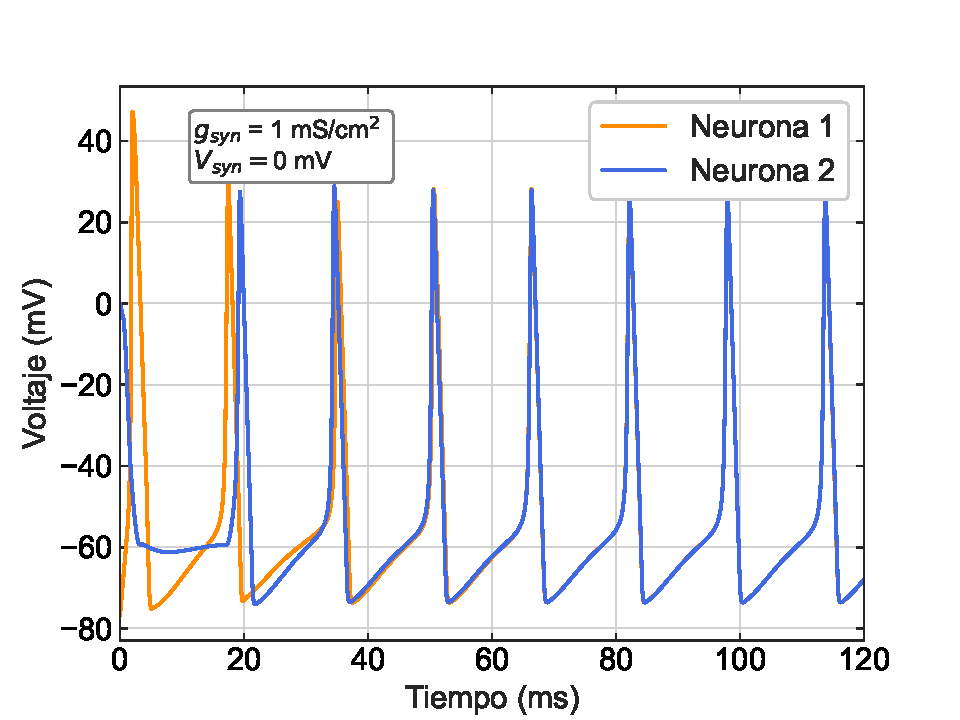
\includegraphics[width=\textwidth]{Figuras/V_vs_t_1_0.pdf}
    \end{subfigure}
\caption{Potencial de las neuronas 1 y 2 en función del tiempo con acople sináptico $g_{syn} = 1 \text{mS}/\text{cm}^2$ e interacción sináptica exitatoria $V_{syn}=0 mV$.} 
\label{fig:V_vs_t_conacople_ext}
\end{figure}
\begin{figure}[H]
    \centering
    \begin{subfigure}[b]{\linewidth}
        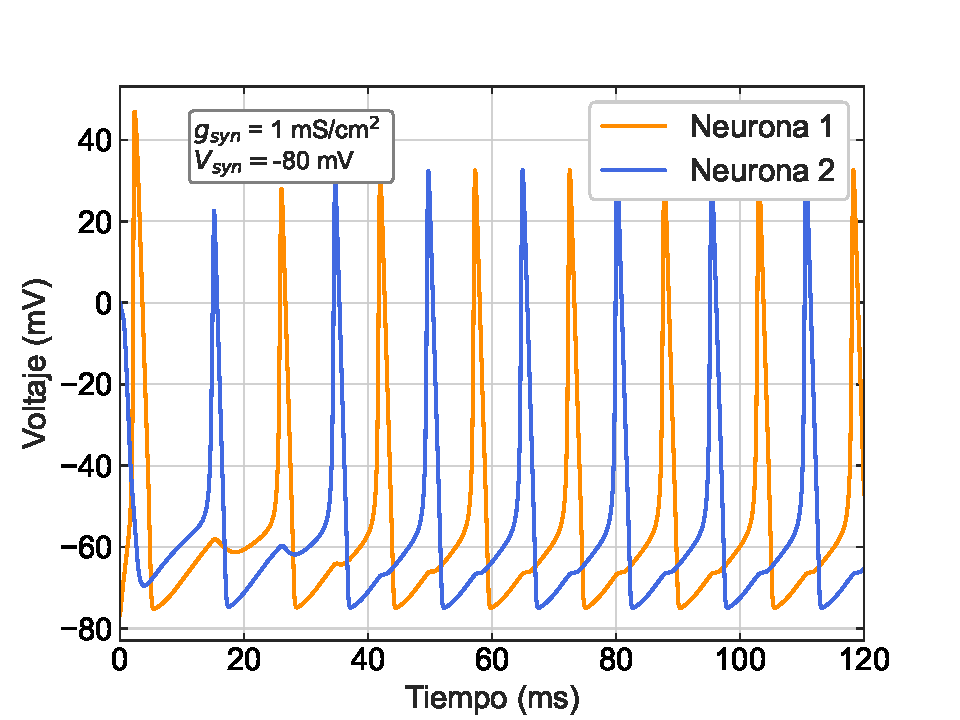
\includegraphics[width=\textwidth]{Figuras/V_vs_t_1_-80.pdf}
    \end{subfigure}
    \caption{Potencial de las neuronas 1 y 2 en función del tiempo con acople sináptico $g_{syn} = 1 \text{mS}/\text{cm}^2$ e interacción sináptica inhibitoria $V_{syn}= -80 mV$.} 
    \label{fig:V_vs_t_conacople_inh}
\end{figure}

Se estudió el desfasaje y la tasa de disparo de las neuronas en función de $g_{syn}$ para interacciones exitatorias ó inhibitorias. Para esto, se tomó $g_{syn}$ entre $0$ y $1 ~ \text{mS}/\text{cm}^2$ y se simuló el potencial de cada neurona durante $1500$ ms donde empíricamente se vio que el sistema llegaba a un estado estacionario. Para ambos estudios se tomaron los últimos diez picos de voltaje de cada neurona. 

El resultado del desfasaje se muestra en la Fig. \ref{fig:desfasaje} donde obtuvo que para todo valor de $g_{syn}>0$ en el caso exitatorio el desfasaje es nulo (neuronas se sincronizan en fase) y para el caso inhibitorio el desfasaje es $\pi$ (neuronas se sincronizan en contrafase). Cuando $g_{syn} = 0$, no hay acople, las neuronas no se sincronizan y el desfasaje queda determinado por las condiciones iniciales de cada neurona.

En la Fig. \ref{fig:frecuencia} se muestran las curvas de la tasa de disparo en función de $g_{syn}$. Se observa que tanto para la interacción exitatoria como inhibitoria la tasa de disparo decae con $g_{syn}$, y con mayor pendiente (negativa) en la interacción exitatoria. Se destaca que aumentar el acople disminuye la tasa de disparo en cualquiera de las dos interacciones pero esta disminución es aún mayor cuando la interacción es exitatoria.

\begin{figure}[ht]
    \centering
         \begin{subfigure}[b]{\linewidth}
            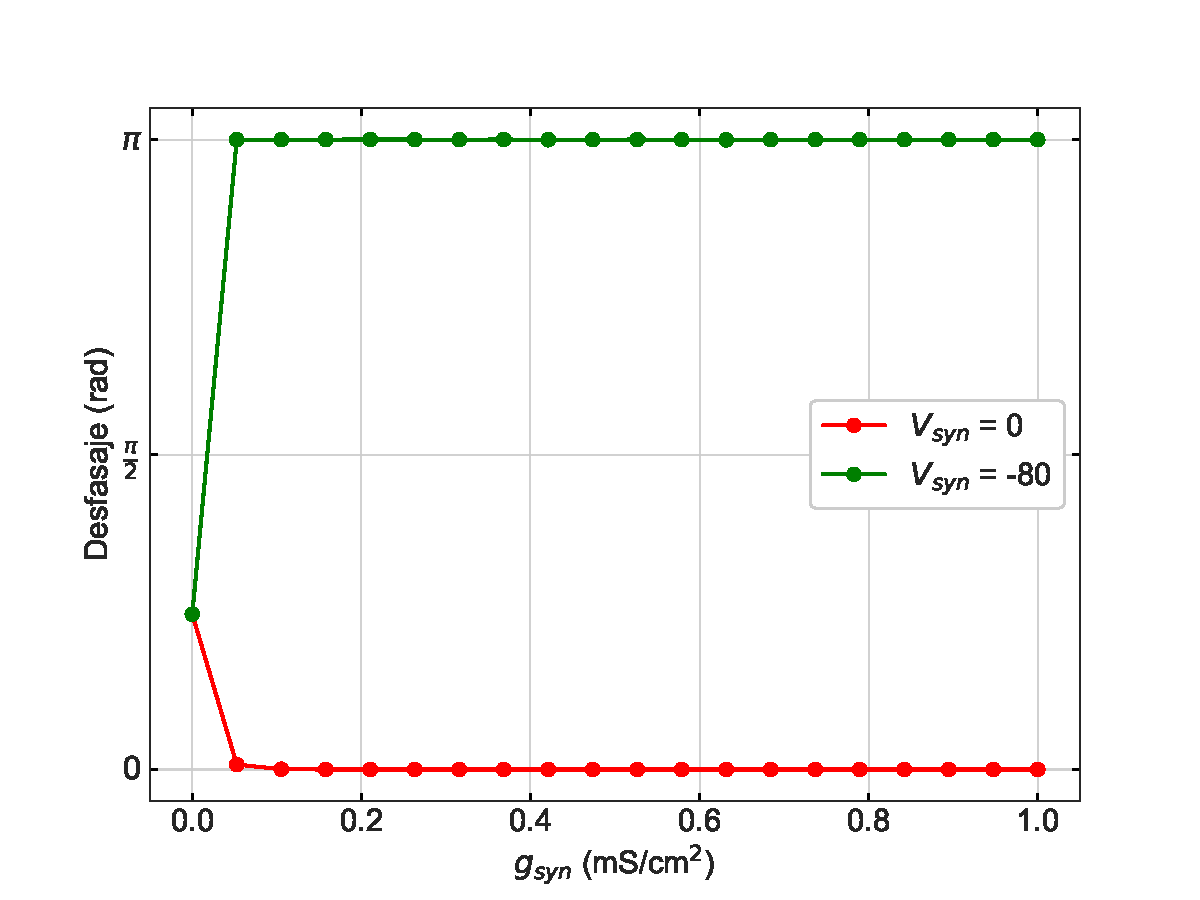
\includegraphics[width=\textwidth]{Figuras/desfasaje_vs_gsyn.pdf}
         \end{subfigure}
    \caption{Desfasaje entre las neuronas 1 y 2 en función del acople sináptico $g_{syn}$.} 
    \label{fig:desfasaje}
\end{figure}

\begin{figure}[ht]
    \centering
         \begin{subfigure}[b]{\linewidth}
            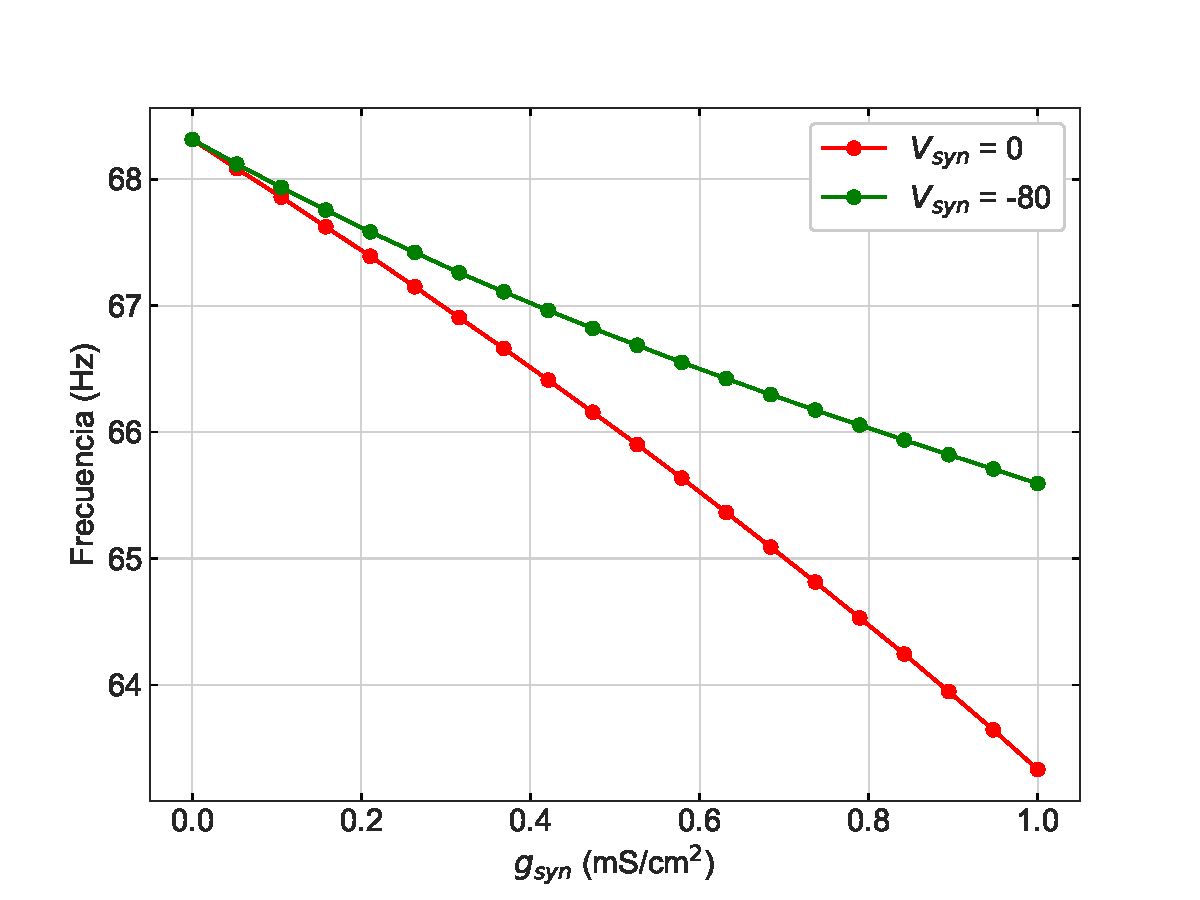
\includegraphics[width=\textwidth]{Figuras/frecuencia_vs_gsyn.pdf}
         \end{subfigure}
    \caption{Tasa de disparo de las neuronas 1 y 2 en función del acople sináptico $g_{syn}$.} 
    \label{fig:frecuencia}
\end{figure}

\newpage

\section{Sistema con dos poblaciones de neuronas \label{sec:p2}}

\vspace{0.3cm}

Se tiene un sistema con dos poblaciones de neuronas descritas por un modelo de tasa de disparo con una relación f-I semilineal
\begin{align}
    \left\{
    \begin{aligned}
    \tau \frac{d h_e}{dt} &= -h_e + g_{ee}f_e - g_{ei}f_i + I_e \\
    \tau \frac{d h_i}{dt} &= -h_i + g_{ie}f_e - g_{ii}f_i + I_i,
    \end{aligned}
\right.
\label{ec:sistema}
\end{align}
donde $f_a = S(h_a)$ ($a=e,i$) con $S(x) = x H(x) $ siendo $H$ la función de Heaviside. Dado que las actividades son $h_e, h_i \geq 0$ entonces $H(h_e) = H(h_i) = 1$. Luego, se buscan los puntos fijos del sistema 
\begin{align}
    \left\{
    \begin{aligned}
        \tau \frac{d h_e}{dt} &= -h_e + g_{ee}h_e - g_{ei}h_i + I_e \\
        \tau \frac{d h_i}{dt} &= -h_i + g_{ie}h_e - g_{ii}h_i + I_i 
    \end{aligned}
    \right.
    \label{ec:sistema2}
\end{align}
el cual se puede escribir de forma matricial como 
\begin{equation}
    \tau \frac{d \vec{h}}{dt} = \boldsymbol{G} \vec{h} + \vec{I}
    \label{ec:sistemamatrix}
\end{equation}
con 
\[
\vec{h} = \begin{pmatrix} h_e \\ h_i \end{pmatrix}, \hspace{0.3cm}
\boldsymbol{G}= \begin{pmatrix} g_{ee} - 1 & -g_{ei} \\ g_{ie} & -1-g_{ii} \end{pmatrix}, \hspace{0.3cm}
\vec{I} = \begin{pmatrix} I_e \\ I_i \end{pmatrix}
\]

En el punto fijo tenemos que $ \frac{d \vec{h}}{dt}=0 $, es decir, estamos buscando las nulclinas para $h_e$ y $h_i$. Pidiendo esta condición, el sistema (\ref{ec:sistemamatrix}) tendrá solución cuando $\text{det}(\boldsymbol{G}) \neq 0$ y resolviendo el sistema de ecuaciones, los valores de las actividades en el punto fijo $h_e^*$ y $h_i^*$ resultan

\begin{align}
    \left\{
    \begin{aligned}
        h_e^* &= \frac{ (1+g_{ii}) I_e - g_{ei}I_i }{\text{det}(\boldsymbol{G})} \\
        h_i^* &= \frac{ g_{ie} I_e - (g_{ee}-1)I_i }{\text{det}(\boldsymbol{G})}
    \end{aligned}
    \right.
    \label{ec:puntofijo}
\end{align}

Ahora como $h_e,h_i > 0$, si $\text{det}(\boldsymbol{G}) > 0$ tenemos las siguientes condiciones
\begin{align}
    \left\{
    \begin{aligned}
        I_i &< I_e \frac{1+g_{ii}}{g_{ei}}\\
        I_i &< I_e \frac{g_{ie}}{g_{ee}-1}
    \end{aligned}
    \right.
\end{align}

Por otro lado, si $\text{det}(\boldsymbol{G}) < 0$ tenemos las siguientes condiciones
\begin{align}
    \left\{
    \begin{aligned}
        I_i &> I_e \frac{1+g_{ii}}{g_{ei}}\\
        I_i &> I_e \frac{g_{ie}}{g_{ee}-1}
    \end{aligned}
    \right.
\end{align}

La estabilidad del punto de equilibrio está dada por la parte real de los autovalores del jacobiano $\boldsymbol{J}$ del sistema (\ref{ec:sistema}) evaluado en $\vec{h}^*$. Solo en el caso que ambos autovalores tengan parte real negativa, el punto fijo es estable. El jacobiano asociado al sistema (\ref{ec:sistema}) evaluado en $\vec{h}^*$ es 
\[
\boldsymbol{J}|_{\vec{h}^*} = \frac{1}{\tau}\begin{pmatrix} g_{ee} - 1 & -g_{ei} \\ g_{ie} & -1-g_{ii} \end{pmatrix},
\]
cuyos autovalores son
\begin{equation}
    \lambda_{1,2} = \frac{1}{2\tau} \biggr( \text{Tr}(J) \pm \sqrt{ (\text{Tr}(J))^2 - 4~\text{det}(J) } \biggr).
    \label{ec:autovalores}
\end{equation}
En este caso $\boldsymbol{J}$ coincide con $\boldsymbol{G}$ porque el sistema es lineal en $h_e, h_i$.

Se analiza la Ec. (\ref{ec:autovalores}) por casos. Si $\text{det}(\boldsymbol{J}) > 0$ el valor dentro de la raíz es siempre menor a $\text{Tr}(\boldsymbol{J})$. Luego, esto implica que, si los autovalores son reales, es decir, 
\begin{equation}
    \text{Tr}(\boldsymbol{J})^2 > 4~\text{det}(\boldsymbol{J}), 
\end{equation}
si $\text{Tr}(\boldsymbol{J}) > 0$ entonces $ \lambda_{1,2} > 0 $ y si $\text{Tr}(\boldsymbol{J}) < 0$ entonces $ \lambda_{1,2} < 0 $. Si los autovalores son complejos el signo de la traza directamente es el signo de la parte real del autovalor. Por lo tanto, para que la solución sea estable cuando $\text{det}(\boldsymbol{J}) > 0$,  $\text{Tr}(\boldsymbol{J}) < 0$. 

Por otro lado, cuando $\text{det}(\boldsymbol{J}) < 0$ los autovalores serán reales y uno será positivo y otro negativo, lo que implica que la solución no puede ser estable.

Entonces, se mostró que $\text{Tr}(\boldsymbol{J}) < 0$ y $\text{det}(\boldsymbol{J}) > 0$ implica estabilidad. La condición para este problema entonces está dada por
\begin{align}
    \left\{
    \begin{aligned}
        \text{Tr}(\boldsymbol{J}) & = g_{ee} - g_{ii} -2 < 0, \\
        \text{det}(\boldsymbol{J}) &= (g_{ee} -1)(-1-g_{ii}) +g_{ei}g_{ie} > 0.
    \end{aligned}
    \right.
\end{align}
Además, si los autovalores son reales y negativos, el comportamiento de la solución es exponencial decreciente hacia el equilibrio, mientras que si son complejos el comportamiento cerca del equilibrio será oscilatorio modulado por una exponencial decreciente.

Se destaca que la estabilidad del punto solo depende de las constantes de interacción sináptica mientras que los valores de $\vec{h}^*$ dependen de estas constantes y de las corrientes $I_e$ e $I_i$.

%Sean $\lambda_1$ y $\lambda_2$ los autovalores de $\boldsymbol{J}$ sabemos que $\text{det}(\boldsymbol{J}) = \lambda_1\lambda_2$ y $\text{Tr}(\boldsymbol{J}) = \lambda_1 + \lambda_2$. Si $\lambda_1$ y $\lambda_2$ son complejos deben ser un par complejo conjugado.


% Bibliography
%\renewcommand*{\bibfont}{\normalsize}
%\bibliography{Redes}

% Full bibliography added automatically for Optics Letters submissions; the following line will simply be ignored if submitting to other journals.
% Note that this extra page will not count against page length
%\bibliographyfullrefs{Redes}


\centerline{\rule{0.95\linewidth}{0.6pt}}

\clearpage 

\begin{onecolumn} % Activa una sola columna para el apéndice
\appendix
\section{Apéndice}

\begin{lstlisting}[language=Python, caption={Implementación del método Runge-Kutta 4.}, label=python-code]

import numpy as np

def rk4(funcs, y0, t0, dt):
    k1 = np.array([func(t0, y0) for func in funcs])
    k2 = np.array([func(t0 + dt/2, y0 + dt/2 * k1) for func in funcs])
    k3 = np.array([func(t0 + dt/2, y0 + dt/2 * k2) for func in funcs])
    k4 = np.array([func(t0 + dt, y0 + dt * k3) for func in funcs])

    y_new = y0 + dt/6 * (k1 + 2*k2 + 2*k3 + k4)
    return y_new
\end{lstlisting}

\begin{lstlisting}[language=Python, caption={Implementación del modelo de una neurona de Hodgkin y Huxley.}, label=python-code]

import numpy as np

#Constantes 
gna = 120 #mS/cm2
gk = 36 #mS/cm2
gcl = 0.3 #mS/cm2
Vna = 50 #mV
Vk = -77 #mV
Vcl = -54.4 #mV
C = 1 #muF/cm2
Iext = 10 #muA/cm2
gsyn = 4
ts = 3 #ms
Vsyn = -80 #mV /-80 mV
tau = 3 #ms

# Definicion de las ecuaciones diferenciales
def n0(V):
    an = 0.01*(V+55)/(1-np.exp((-V-55)/10))
    bn = 0.125*np.exp((-V-65)/80)
    return an/(an+bn)
def tn(V):
    an = 0.01*(V+55)/(1-np.exp((-V-55)/10))
    bn = 0.125*np.exp((-V-65)/80)
    return 1/(an+bn)
def m0(V):
    am = 0.1*(V+40)/(1-np.exp((-V-40)/10))
    bm = 4*np.exp((-V-65)/18)
    return am/(am+bm)
def tm(V):
    am = 0.1*(V+40)/(1-np.exp((-V-40)/10))
    bm = 4*np.exp((-V-65)/18)
    return 1/(am+bm)
def h0(V):
    ah = 0.07*np.exp((-V-65)/20)
    bh = 1/(1+np.exp((-V-35)/10))
    return ah/(ah+bh)
def th(V):
    ah = 0.07*np.exp((-V-65)/20)
    bh = 1/(1+np.exp((-V-35)/10))
    return 1/(ah+bh)
def s0(V_pre):
    return 0.5*(1+np.tanh(V_pre/5))
def f_s(s, Vpre):
    return (s0(Vpre) - s)/ts
def f_n(n, V):
    return (n0(V) - n)/tn(V)
def f_m(m, V):
    return (m0(V) - m)/tm(V)
def f_h(h, V):
    return (h0(V) - h)/th(V)
def f_V(s, n, m, h, V):
    return (Iext - gk*(n**4)*(V-Vk) - gna*(m**3)*(h)*(V-Vna) - 
    gcl*(V-Vcl) - gsyn*(s)*(V-Vsyn))/C
funcs = [
    lambda t, y: f_s(y[0], y[9]) ,
    lambda t, y: f_s(y[1], y[8]) ,
    lambda t, y: f_n(y[2], y[8]) ,
    lambda t, y: f_n(y[3], y[9]) ,
    lambda t, y: f_m(y[4], y[8]) ,
    lambda t, y: f_m(y[5], y[9]) ,
    lambda t, y: f_h(y[6], y[8]) ,
    lambda t, y: f_h(y[7], y[9]) ,
    lambda t, y: f_V(y[0], y[2], y[4], y[6], y[8])  ,
    lambda t, y: f_V(y[1], y[3], y[5], y[7], y[9])  ,
]
\end{lstlisting}
    
\begin{lstlisting}[language=Python, caption={Simulación de una interacción exitatoria o inhibitoria entre dos neuronas de Hodgkin y Huxley para un dado valor de $g_{syn}$.}, label=python-code]

import numpy as np
import matplotlib.pyplot as plt
import HH_neuron as hh
import rk4 as rk4
import seaborn as sns
#sns.set(context='paper')
sns.axes_style("whitegrid")
sns.set_style("ticks")

#Parametros de la simulacion: y = [s1, s2, n1, n2, m1, m2, h1, h2, V1, V2]
y_initial = np.array([hh.s0(hh.Vk), 0, hh.n0(hh.Vk), 0, hh.m0(hh.Vk), 0, 
hh.h0(hh.Vk), 0, hh.Vk, 0])
t_initial = 0.0 #ms
t_final = 500 #ms
time_step = 0.01 #ms

hh.gsyn = 1 #mS/cm2
hh.Vsyn = 0 #mV

#Simulacion
steps = int(t_final/time_step) 
t_values = np.empty(steps)
V1_values = np.empty(steps)
V2_values = np.empty(steps)

t = t_initial
y = y_initial

for i in range(steps):
    # Aplicar un paso de Runge-Kutta de orden 4
    y = rk4.rk4(hh.funcs, y, t, time_step)

    t_values[i] = t
    V1_values[i] = y[8]
    V2_values[i] = y[9]
    
    t += time_step

#Ploteo
plt.plot(t_values, V1_values, color='darkorange',  label = "Neurona 1")
plt.plot(t_values, V2_values, color='royalblue', label = "Neurona 2")
plt.xlabel("Tiempo (ms)", fontsize=15)
plt.ylabel("Voltaje (mV)", fontsize=15)
plt.xticks(rotation=0, fontsize=15, color='black')
plt.yticks(fontsize=15, color='black')
plt.tick_params(direction='in', top=True, right=True, left=True, bottom=True)
plt.legend(fontsize=15, framealpha=1, loc = 'upper right')
plt.xlim(0, 120)
plt.grid(True, linewidth=0.5, linestyle='-', alpha=0.9)
plt.annotate('$g_{syn}$ = ' + str(hh.gsyn) + ' mS/cm$^2$ \n$V_{syn} = $' 
+ str(hh.Vsyn) + ' mV', xy=(0.1, 0.85), xycoords='axes fraction', fontsize=12, 
bbox=dict(boxstyle='round,pad=0.2', edgecolor='grey', facecolor='white'))

plt.savefig(f"../Redes-Neuronales/Practica_2/resultados/V_vs_t_{hh.gsyn}_
{hh.Vsyn}.pdf")
plt.savefig(f"../Redes-Neuronales/Practica_2/resultados/V_vs_t_{hh.gsyn}_
{hh.Vsyn}.png", dpi=600)

\end{lstlisting}
    
\begin{lstlisting}[language=Python, caption={Código para calcular el desfasaje entre dos neuronas de Hodgkin y Huxley y la tasa de disparo, para un dado valor de $g_{syn}$} en una interacción exitatoria o inhibitoria , label=python-code]

import numpy as np
import matplotlib.pyplot as plt
import HH_neuron as hh
import rk4 as rk4
import seaborn as sns
from scipy.signal import find_peaks

#sns.set(context='paper')
sns.axes_style("whitegrid")
sns.set_style("ticks")
fig1, ax1 = plt.subplots(figsize=(8,6)) 
fig2, ax2 = plt.subplots(figsize=(8,6)) 

for Vsyn in [0, -80]: #mV
    gsyns = np.linspace(0, 1, 20) #mS/cm2
    f = []
    shift = []
    hh.Vsyn = Vsyn
    print(hh.Vsyn)
    for gsyn in gsyns:
        hh.gsyn = gsyn
        print(hh.gsyn)
        # Valores iniciales: y = [s1, s2, n1, n2, m1, m2, h1, h2, V1, V2]
        y_initial = np.array([hh.s0(hh.Vk), 0, hh.n0(hh.Vk), 0, hh.m0(hh.Vk), 0, 
        hh.h0(hh.Vk), 0, hh.Vk, 0])
        t_initial = 0.0 #ms
        t_final = 1500 #ms
        time_step = 0.01 #ms

        #Simulacion
        steps = int(t_final/time_step) 
        t_values = np.empty(steps)
        V1_values = np.empty(steps)
        V2_values = np.empty(steps)

        t = t_initial
        y = y_initial

        for i in range(steps):
            # Aplicar un paso de Runge-Kutta de orden 4
            y = rk4.rk4(hh.funcs, y, t, time_step)

            t_values[i] = t
            V1_values[i] = y[8]
            V2_values[i] = y[9]
            
            t += time_step
                
        peaks1, _ = find_peaks(V1_values, height=0) 
        peaks2, _ = find_peaks(V2_values, height=0) 
        
        # Encontrar los picos dentro del rango de interes
        peaks1 = peaks1[-10:]
        peaks2 = peaks2[-10:]
        T1 = (t_values[peaks1[1:]] - t_values[peaks1[:-1]])
        T2 = (t_values[peaks2[1:]] - t_values[peaks2[:-1]])

        T = (np.concatenate((T1,T2))).mean()
        f.append(1.0/(T*1e-3)) #Hz
        Tdiff = np.abs(t_values[peaks1] - t_values[peaks2])
        Tshift = Tdiff.mean()
        shift.append((Tshift%T)/T * 2 * np.pi) 

    if(Vsyn == 0):
        color = 'r'
    else:
        color = 'g'

    # Ploteo para la figura 1
    ax1.plot(gsyns, f, "-o", color= color,  label = "$V_{syn}$ = " + str(Vsyn) )
    ax1.set_xlabel("$g_{syn}$ (mS/cm$^2$)", fontsize=15)
    ax1.set_ylabel("Frecuencia (Hz)", fontsize=15)
    ax1.tick_params(direction='in', top=True, right=True, left=True, bottom=True)
    ax1.legend(fontsize=15, framealpha=1)
    ax1.tick_params(axis='x',rotation=0, labelsize=18, color='black')
    ax1.tick_params(axis='y', labelsize=18, color='black')
    #ax1.set_xlim(0, 200)
    ax1.grid(True, linewidth=0.5, linestyle='-', alpha=0.9)
    #ax1.annotate('$g_{syn}$ = ' + str(hh.gsyn) + ' mS/cm$^2$ \n$V_{syn} = $' 
    + str(hh.Vsyn) + ' mV', xy=(0.1, 0.825), xycoords='axes fraction', 
    fontsize=12, bbox=dict(boxstyle='round,pad=0.2', edgecolor='grey',
    facecolor='white'))
    # Guardar figura 1
    fig1.savefig(f"../Redes-Neuronales/Practica_2/resultados/frecuencia_vs_gsyn.pdf")
    fig1.savefig(f"../Redes-Neuronales/Practica_2/resultados/frecuencia_vs_gsyn.png",
    dpi=600)

    # Ploteo para la figura 2
    ax2.plot(gsyns, shift, "-o", color= color, label = "$V_{syn}$ = " + str(Vsyn))
    ax2.set_xlabel("$g_{syn}$ (mS/cm$^2$)", fontsize=15)
    ax2.set_ylabel("Desfasaje (rad)", fontsize=15)
    ax2.tick_params(direction='in', top=True, right=True, left=True, bottom=True)
    ax2.set_yticks([0, np.pi/2, np.pi])
    ax2.set_yticklabels(["$0$",  r"$\frac{\pi}{2}$", r"$\pi$"])
    ax2.legend(fontsize=15, framealpha=1)
    ax2.tick_params(axis='x',rotation=0, labelsize=18, color='black')
    ax2.tick_params(axis='y', labelsize=18, color='black')
    ax2.grid(True, linewidth=0.5, linestyle='-', alpha=0.9)
    # Guardar figura 2
    fig2.savefig(f"../Redes-Neuronales/Practica_2/resultados/desfasaje_vs_gsyn.pdf")
    fig2.savefig(f"../Redes-Neuronales/Practica_2/resultados/desfasaje_vs_gsyn.png",
    dpi=600)
\end{lstlisting}
\end{onecolumn}



\end{document}


